\textbf{\hypertarget{P10}{[\,Suggested Time: 25 mins \textbar \, Total Marks: 10 \textbar \, Extensions\,]}}\\
%%%%%Question i, Proving the parallel eff. resistance equation%%%%%
\textit{\textbf{(i)} Deduce that the effective resistance, \(R_{eff}\), of n parallel resistors is \(\displaystyle R_{eff} = \left(\sum_{i = 1}^{n} \frac{1}{R_{i}}\right)^{-1}\)} \qnmark{5} \\

%%%%%%%%%%%%%%%%%%
%%%%%Solution%%%%%
%%%%%%%%%%%%%%%%%%

%\begin{comment}

%%%%%Electricity laws in a parallel circuit%%%%%
\begin{gather*}
    Total \; current \; in \; a \; parallel \; circuit, \; \displaystyle I_{T} = \sum_{i=1}^{n} I_{i} \hspace*{10pt} (KCL) \\
    Voltage \; in \; a \; parallel \; circuit \; \displaystyle V_{T} = V_{1} = V_{2} = V_{3} \; \cdots \onemark \\
\end{gather*}

\textit{By Ohm's Law, V = IR, it is trivial that}
\begin{equation*}
    \displaystyle I_{1} = \frac{V_{1}}{R_{1}}, I_{2} = \frac{V_{2}}{R_{2}}, \cdots, I_{n} = \frac{V_{n}}{R_{n}} \onemark
\end{equation*}

\textit{Note that since $\displaystyle V_{T} = V_{1} = V_{2} = V_{3} \; \cdots$ , we can rewrite the equations above as}
\begin{equation*}
    \displaystyle I_{1} = \frac{V_{T}}{R_{1}}, I_{2} = \frac{V_{T}}{R_{2}}, \cdots, I_{n} = \frac{V_{T}}{R_{n}} \onemark
\end{equation*}


%%%%%Proving the equation in the question%%%%%
\textit{Using KCL and the equations that we had derived, we can see that}
\begin{align*} %% Finding I_{T}
    \displaystyle I_{T} &= \sum_{i=1}^{n} \frac{V_{T}}{R_{i}} \\
    \displaystyle       &= V_{T} \sum_{i=1}^{n} \frac{1}{R_{i}} \onemark \\
\end{align*}
\textit{By Ohm's law,}
\begin{align*}
    \displaystyle R_{eff} &= \frac{V_{T}}{I_{T}} \\
    \displaystyle         &= \frac{V_{T}}{\displaystyle V_{T}\sum_{i=1}^{n} \frac{1}{R_{i}}} \\
    \displaystyle         &= \frac{1}{\displaystyle \sum_{i=1}^{n} \frac{1}{R_{i}}} \\
    \displaystyle         &= \left(\sum_{i=1}^{n} \frac{1}{R_{i}}\right)^{-1} \tag*{\qedsymbol} \\ \onemark
\end{align*}

%\end{comment}

\newpage \ \newpage %Don't Comment

%%%%%Question iia, finding the eff. resistance of a parallel resistor system%%%%%
\begin{center}
    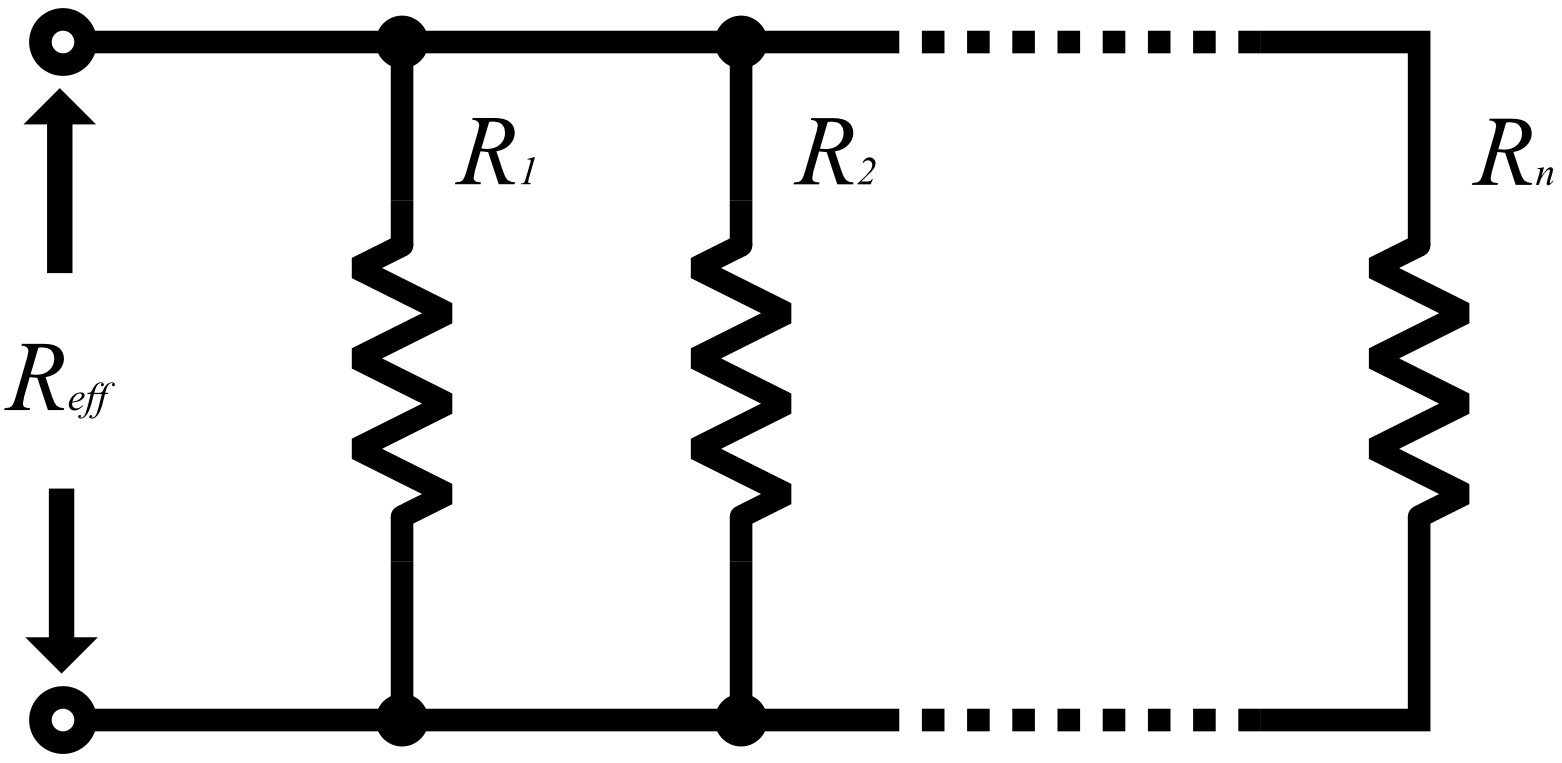
\includegraphics[scale=0.25]{Question 10iia - Circuit Diagram.jpg}
\end{center}
\textit{\textbf{(ii)(a)} Hence or otherwise, find the effective resistance of the circuit shown above. \\
        \hspace*{35pt} Where \(R_{1} = \sqrt{1}+\sqrt{2}, R_{2} = \sqrt{2}+\sqrt{3}, R_{3} = \sqrt{3}+\sqrt{4} \; \cdots\) \\
        \hspace*{35pt} \textbf{Leave your answers in exact values}, and in terms of n.
} \qnmark{4} \\

%%%%%%%%%%%%%%%%%%
%%%%%Solution%%%%%
%%%%%%%%%%%%%%%%%%

%\begin{comment}

%%%%%Representing the effective resistance of the circuit with (i)%%%%%
\textit{We can see that the resistance of the resistors follow a series with a general term of}
\begin{equation*}
    \displaystyle R_{n} = \sqrt{n}+\sqrt{n+1} \onemark \\
\end{equation*}

\textit{Using the equation in part \textbf{(i)},}
\begin{align*}
    \displaystyle R_{eff} &= \left(\sum_{\alpha = 1}^{n} \frac{1}{\sqrt{\alpha}+\sqrt{\alpha+1}}\right)^{-1} \\
    \displaystyle         &= \left(\sum_{\alpha = 1}^{n} \frac{\sqrt{\alpha}-\sqrt{\alpha+1}}{\alpha-\alpha-1}\right)^{-1} \\
    \displaystyle         &= \left(\sum_{\alpha = 1}^{n} \left(\sqrt{\alpha+1}-\sqrt{\alpha}\right)\right)^{-1} \onemark \\
\end{align*}

%%%%%Evaluating the sum%%%%%
\textit{Evaluating the sum}
\begin{align*}
    \sum_{\alpha = 1}^{n} \left(\sqrt{\alpha+1}-\sqrt{\alpha}\right) =& \left(\sqrt{2}-\sqrt{1}\right) + \\
                                                                      & \left(\sqrt{3}-\sqrt{2}\right) + \\
                                                                      & \left(\sqrt{4}-\sqrt{3}\right) + \\
                                                                      & \vdots \\
                                                                      & \left(\sqrt{n+1}-\sqrt{n}\right) \\
                                                                     =& \sqrt{n+1}-1 \onemark
\end{align*}

\newpage

%%%%%Finding the effective resistance%%%%%
\textit{Substituting the sum back into \(R_{eff}\)}
\begin{equation*}
    \displaystyle \therefore R_{eff} = \frac{1}{\sqrt{n+1}-1} \onemark \\
\end{equation*} \\
\textit{The effective resistance of the circuit is $\displaystyle \frac{1}{\sqrt{n+1}-1}$, \\
        where n is the number of resistors
}

%\end{comment}

\newpage %% Don't Comment
%\ \newpage

%%%%%Question iib, proving if this is converging series%%%%%
\textit{\textbf{(ii)(b)} Explain, with relevant workings, if the effective resistance of the circuit \\
        \hspace*{40pt} will approach a unique value as more resistors are added into the circuit.
} \qnmark{1} \\

%%%%%%%%%%%%%%%%%%
%%%%%Solution%%%%%
%%%%%%%%%%%%%%%%%%

%\begin{comment}

\textit{from (ii)(a), \(\displaystyle R_{eff} = \frac{1}{\sqrt{n+1}-1}\)} \\
\begin{align*}
    \displaystyle As \; n \rightarrow \infty, \; \sqrt{n+1}-1 &\rightarrow \infty \\
    \displaystyle                      \frac{1}{\sqrt{n+1}-1} &\rightarrow 0 \\
    \displaystyle                          \therefore R_{eff} &\rightarrow 0 \onemark \\
\end{align*}
\textit{Yes, \(R_{eff}\) approaches the value 0 as more resistors are added into the circuit}


%\end{comment}